The previous chapter introduced a model for a decentralised location proof system. This chapter will present an evaluation of the model with respect to the design goals defined in section \ref{sec:design_goals}.

\section{OTIT conformance}
As explained in section \ref{ssec:otit}, the OTIT model \cite{otit} defines 8 desirable properties of a lcoation proof system. The model introduced in chapter \ref{ch:design} is evaluated with respect to OTIT below.

\subsection{Chronological}
The chronological property of OTIT states that location proofs should be ordered according to the sequence of their creation.

This property is not enforced at the time of transaction publication in this system. This is to avoid revealing any transaction information to the miner nodes, therefore preserving the privacy of the transaction owner. Instead, the Chronological property is enforced at the time of verification. The chronological link created by adding $KL_{AT}(ID_{A}[n-1]|ts_A)$ to the published transaction will allow Verifier nodes to prove that the transaction is chronologically ordered. Therefore the system preserves OTIT's ``Chronological'' property.

\subsection{Order preserving}
This property states that the order in which location proofs were entered into the proof chain should be maintained.

In this system, a blockchain is used to store location proof transactions. In a blockchain, new blocks are added in a linear, chronological order, and cannot be modified so long as the majority of miners in the network are honest \cite{blueprint}.

A block consists of a number of transactions. These transactions are included in the block in the order they were received by the miner who solved the proof-of-work for that block. Once the block has been signed into the blockchain, it is impossible for the transactions inside the block to be reordered, assuming the miner network is controlled by a majority of honest nodes.

As a further method of preserving order, each node includes its observed timestamp in its encrypted transaction and link data. This prevents a group of malicious miner nodes from altering the order and timestamp of the transaction before signing it into the blockchain. Therefore the transactions stored in these blocks satisfy the ``Order preserving'' property of OTIT.

\subsection{Verifiable}
This states that a Verifier should be able to verify or reject the claim by the user that he has visited the given location(s).

The sytem described in chapter \ref{ch:design} inherently satisfies this property of OTIT. Verifier nodes may be operated by banks, employers, or other parties who have a vested interest in allowing their customers or employees to be able to prove their location. These Verifiers can verify or reject a mobile nodes claimed location by examining the nodes chronological link of transactions (as shown in figure \ref{fig:tree}). The Verifier will revursively generate and examine this tree until it can conclude whether the transaction chain is valid or not.

\subsection{Tamper evident}
The system is tamper evident, meaning the Verifier is able to detect if the proof chain has been tampered with or modified. If a malicious node creates a successful transaction with an honest node, but modifies the transaction data before publishing, a Verifier node will reject the malicious transaction. This rejection will be on the grounds that the matching transaction, published by the honest node, contains contradictory data.

The design assumes the underlying security of the blockchain, so any malicious miner nodes will not be able to tamper with existing transaction data providing that the majority of CPU power in the mining system is owned by honest miners \cite{bitcoin}. Therefore the tamper evident property is satisfied.

\subsection{Privacy preserved}
This property states that when the proof chain is verified for specific location proofs, privacy must be preserved for the other location proofs within the chain.

In the system, privacy is preserved using \textit{Key Lists} \ref{ssec:key_lists}. Two keys are used for each transaction; $KL_{AT}[n]$ is used to encrypt the \textit{transaction data} for $A$'s $nth$ transaction, and $KL_{AL}[n]$ is used to encrypt the \textit{backwards chronological link} between $A$'s $nth$ transaction and transaction $n-1$.

To control his privacy, a user can choose only to reveal $KL_{AL}[n]$ for a specific transaction $n$. This may be useful if a user does not wish to reveal transaction data for transactions created within a certain distance of his house, for example. Hiding $KL_{AT}[n]$ while revealing $KL_{AL}[n]$ has the advantage of preserving the user's privacy while maintaining a clear backwards chronological link of transactions for the Verifier to follow. This simulatneously preserves both privacy and chronological integrity.

\subsection{Selective in-sequence privacy}
This is the requirement that the user must be able to choose not to reveal certain location proofs within the proof chain when seeking verification. The system satisfies this property by using \textit{Key Packets} (section \ref{sssec:key_packets}).

A \textit{sub-set} of size $m$ of a node $A$'s proof chain, beginning at proof $n$, contains all proofs in the sequence $ID_{A}[n-m] - ID_{A}[n]$. Every transaction in this chain is split into two parts (a transaction data and link data part), and separately encrypted. If a node reveals keys for a verifier decrypt all transactions in the sequence $ID_{A}[n-m] - ID_{A}[n]$, it will not be possible for the verifier to discover transaction $ID_{A}[n-m-1]$, or any transaction outside the sequence $ID_{A}[n-m] - ID_{A}[n]$.

By encrypting each transaction with a different pair of keys, this system satisfies OTIT's ``selective in-sequence privacy'' property.

\subsection{Privacy protected chronology}
This property of OTIT states that the location proof system should ensure that the user does not hide important information from the items within the subset of the proof chain. In this system, it is impossible by design to hide important information, due to the use of backwards chronological linking between transactions. 

\subsection{Convenience and derivability}
This requirement states that the system must ensure that the user does not burden the Verifier with a large amount of data to analyse in order to verify the user's location.

In this system, the data is stored in a central blockchain that the Verifier has access to, and the user provides the Verifier  with decryption keys and indexes into just a sub-section of this data. Therefore the data sent to from the user to the Verifier, $KP_{An}$, is quite small in size.

The Verifier has the freedom to decide how comprehensively to investigate the users data; It can decide how far to recurse while investigating the tree of alibi relationships. This property of OTIT is therefore satisfied by allowing the Verifier to decide how complex the verification process needs to be.

\section{Threat analysis}
\subsection{False presence}
In a false presence attack, a dishonest user attempts to obtain a location proof for a false location.

In this system, any dishonest user attempting to obtain a location proof with an honest alibi will not succeed, as the honest alibi will abort the exchange (see section \ref{ssec:aborting_exchanges}). A dishonest user who publishes a transaction onto the blockchain with a fabricated alibi will also not succeed, as the transaction will be rejected during verification if a Verifier can't find the matching alibi transaction. The system is therefore not vulnerable to a false presence attack.

\subsection{Malicious intruders}
A malicious intruder offers to help another user to prove a false location, but doesn't prove a false location for himself.

In the context of this system, a malicious intruder may collude with another user to prove a false location, by acting as an alibi. These transactions will be successfully published onto the blockchain. However, if this user attempts to have his transaction chain verified, a Verifier will quickly notice the lack of credible alibis in the proof chain, indicating malicious activity, and reject the proof request. A sample tree of a node with uncredible alibis is shown in figure \ref{fig:uncredible_tree}. This avoids a malicious intruder vulnerability.

\begin{figure}[H]
\begin{center}
\resizebox {0.5\columnwidth} {!} {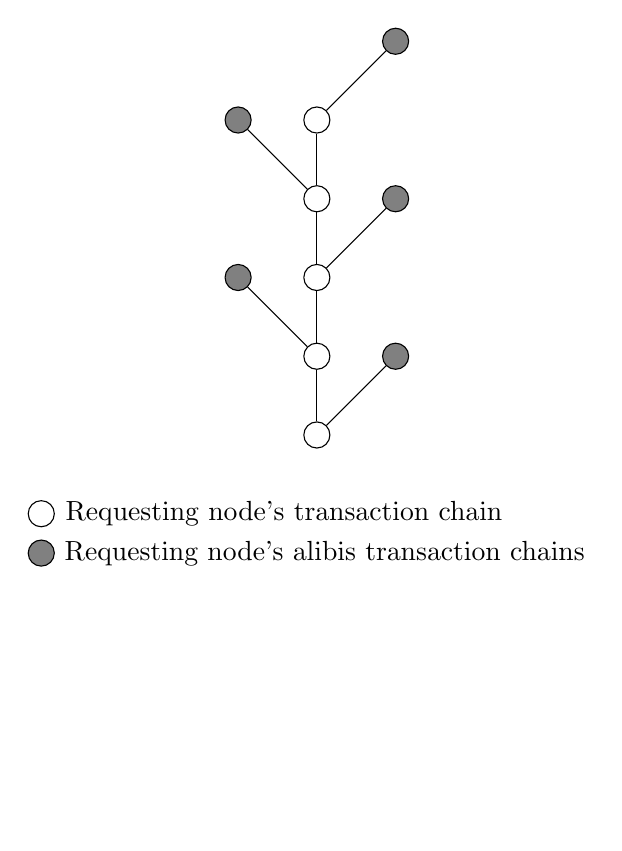
\begin{tikzpicture}[every node/.style={draw,shape=circle,fill=black}]

\node[fill=white] (A) at (0,0) {};
\node[fill=white] (B) at (0,1) {};
\node[fill=white] (C) at (0,2) {};
\node[fill=white] (D) at (0,3) {};
\node[fill=white] (E) at (0,4) {};

\node[fill=white,label=right:Requesting node's transaction chain] (L1) at (-3.5,-1) {};
\node[fill=gray,label=right:Requesting node's alibis transaction chains] (L2) at (-3.5,-1.5) {};

\draw (A) -- (B) (B) -- (C) (C) -- (D) (D) -- (E);

\node[fill=gray] (F) at (1,1) {};
\draw (A) -- (F);

\node[fill=gray] (G) at (-1,2) {};
\draw (B) -- (G);

\node[fill=gray] (H) at (1,3) {};
\draw (C) -- (H);

\node[fill=gray] (I) at (-1,4) {};
\draw (D) -- (I);

\node[fill=gray] (J) at (1,5) {};
\draw (E) -- (J);

\end{tikzpicture}}
\vspace{-3cm}
\caption{A proof chain with uncredible alibis}
\label{fig:uncredible_tree}
\end{center}
\end{figure}

\subsection{Curious users}
A curious user is one who learns another users identity by monitoring its location proofs.

Identity discovery is impossible by design in this sytem. By using a different, seemingly random identity for each transaction, it is impossible for a curious user to determine if two transactions belong to the same user or not. It is therefore impossible for a curious user to learn another users identity by monitoring location proofs.

\subsection{Malicious applications}
A malicious application is one that tries to take advantage of a users information as the user seeks verification.

This attack does not affect this system, as a user will only seek verification from applications (verifiers) it deems trustworthy. Verifiers, such as banks or employers, will be known to the user, and therefore trusted. The user also has complete control over which verifiers it chooses to seek verification from, it is not obliged to send verification requests to any verifier.

\subsection{Eavesdroppers}
An eavesdropper intercepts or modifies communication between two honest users. This threat does not affect this system, as ad-hoc bluetooth networks are set up between two mobile nodes advertising their current transaction ID, e.g. $ID_A[n]$. An eavesdropper will not be a member of this ad-hoc network, and therefore cannot modify any communication in the network.

\subsection{Wormhole attacks}
In a wormhole attack, an attacker records network traffic in one location and replays it in another location, at another time.

This attack is not relevant to the system presented in chapter \ref{ch:design}, as this system is decentralised. Any wormhole attack transmissions will simply be ignored by the intended victim.

\subsection{Weak identities}.
In a weak identity attack, a user gives his public key or identity to another colluding user in order to create a location proof.

A weak identity attack will not affect this system. Exchanging public keys or identities between colluding users offers no advantage. This is because the Verifier will ensure that any users requesting verification own the private key corresponding to the public key transferred during the verification request (see section \ref{ssec:verification}).

\subsection{False timestamping}
False timestamping includes backdating and future dating attacks. In a backdating attack, the attacker creates a location proof with a past timestamp. In future dating, the attacker creates a location proof with a future timestamp.

This system is resilient against a false timestamping attack by design. Every transaction is created with a reference to an alibi transaction. If an attacker creates a transaction with a past or future timestamp, the corresponding alibi transaction will contain contradictory information, and a Verifier will disregard it.

\subsection{Implication}
An implication attack occurs when a malicious user, or group of colluding malicious users, create a false location proof for an honest user.

This system is resilient to an implication attack. Location proofs are stored in a public blockchain, but the decryption keys, nonce and public key used to create the transaction all reside with the user who created it. A user cannot be implicated in a location proof without creating the identity used in the proof, and encrypting the transaction data.

It is therefore impossible to implicate an honest user in a location proof, without finding vulnerabilities outside the location proof system (for example by compromising their device).

\subsection{False assertion}
In a false assertion attack, two malicious users collude to create false location proofs for themselves.

It is possible in this system for two malicious users to collude as alibis and publish their transactions on the blockchain. This is allowed because the miner nodes do not know the contents of the data they are signing into the blockchain, as it is encrypted.

Providing that the system is comprised of a majority of honest nodes, this attack will not succeed. It will be obvious to a Verifier after construcing a graph of the nodes alibi transaction (as shown in section \ref{ssec:verification}) that the graph lacks alibi credibility, and therefore two malicious users are likely colluding to create location proofs for themselves. Therefore the system is not vulnerable to this attack.

\subsection{Proof switching}
In a proof switching attack, a malicious user modifies one of its existing honest proofs to spoof a false location.

This is not possible in this system, as the blockchain is used as a tamper-proof method of storing location proofs. Once the proof is included in the blockchain, it cannot be modified.

If the proof has not been added to the blockchain yet, then it is possible for the malicous user to modify it to attempt to spoof a false location. However this attack will not work on this system. Any Verifier will reject the transaction on the grounds that it contains contradictory information to the alibis transaction, which has not been modified.

\subsection{Relay attack}
In a relay attack, a malicious user uses a colluding \textit{proxy user} physically present at the location that the malicious user wishes to create a false proof, to create a location proof with an honest user.

This system is resilient against a most relay attacks. This is because proofs created using a proxy user will be inconsistent with the other proofs in a users proof chain. For example, a user living in New York uses a proxy user to create a proof with a user in London. A Verifier will reject the users claim that it is in London, because of the lack of alibi credibility.

One vulnerability of the system can be called a \textit{complete} relay attack. In a \textit{complete} relay attack, two malicious nodes exist purely for the purpose of proxying location proof. One node, the proxy, will \textit{never} request location proofs for itself. Its only purpose is to proxy exchange data between honest nodes and the other malicious node, the \textit{attacker}.

Resilience against a complete relay attack scenario must be taken out of the scope of this system. 

\subsection{Sybil attack}
A Sybil attack occurs when a single malicious user generates multiple \textit{pseudoidentities}, and begins masquerading as multiple users.

While some studies have been done on Sybil attacks in decentralised systems \cite{sybil}. There are various methods of mitigating against a subil attack, however a solution for the Sybil attack in a decentralised system is considered an open problem. This system is therefore vulnerable to a highly targeted Sybil attack.

